%%%%%%%%%%%%%%%%%%%%%%%%%%%%%%%%%%%%%%%%%%%%%%%%%%%%%%%%%%%%%%%%
%% Proceedings Sample, ProcChap.tex
%% Kluwer Academic Press
%%
%% Prepared by Amy Hendrickson, TeXnology Inc., July 1999.
%%%%%%%%%%%%%%%%%%%%%%%%%%%%%%%%%%%%%%%%%%%%%%%%%%%%%%%%%%%%%%%%

%%%%%
%% LaTeX2e 
%% Uncomment documentclass, 
\documentclass{kapproc} % Computer Modern font calls

%\usepackage[dvipdf]{graphicx}
\usepackage{graphicx}


%% and, optionally, one or more 
%%   of the \usepackage commands below:

%%%%%


%% If you use a font encoding package, please enter it here, i.e.,
%% \usepackage{T1enc}
\usepackage[T1]{fontenc}

%%%%%
%  If you have MathTimes and MathTimesPlus fonts, you
%  may uncomment the line below and use them, but you are
%  not obligated to do so, and most authors do not have
%  these fonts. (You may need to edit m-times.sty to make the
%  font names match those on your system)

%  You must have the MathTimes fonts for this to work. They may be
%  purchased from the Y&Y company, http://www.YandY.com.

%  \usepackage[mtbold,noTS1]{m-times}

%%%%%
% PostScript font calls
%
% If you use the procps PS font file, you may need to edit it
% to make sure the font names match those on your system. See
% the top of the procps.sty file for more info.

  \usepackage{procps} 

%%%%%%%%%%%%%%%%%%%%%%%%%%%%%%%%%%%
%% LaTeX209, uncomment only one:
%% (Make sure documentclass and usepackage commands above are commented out!)
%
%  \documentstyle{kapproc} % Computer Modern fonts
%  \documentstyle[procps]{kapproc} %For PostScript fonts 
%   (MathTimes style is not available for authors using LaTeX2.09)

%%%%%%% Formatting Commands You Can Set or Change ===>>>

%  optional, uncomment to make current time and `draft' appear at
%  bottom of page.
%\draft

%%%% To change footnotes to appear at bottom of page ==>
%% (Default is endnotes that appear at the end of the chapter, above
%%   the references, or whereever \notes is written.)

%% uncomment to make footnote appear at bottom of page:
\let\footnote\savefootnote

%% uncomment if you want footnotetext to appear at the bottom of the page:
%\let\footnotetext\savefootnotetext 

%% uncomment if you want a ruled line above the footnote:
%\let\footnoterule\savefootnoterule 

%%%% <== end footnote changes


%% How many levels of section head would you like numbered?
%% 0= no section numbers, 1= section, 2= subsection, 3= subsubsection
%%==>>
\setcounter{secnumdepth}{2}


%% How many levels of section head would you like to appear in the
%% Table of Contents?
%% 0= chapter titles, 1= section titles, 2= subsection titles, 
%% 3= subsubsection titles.
%%==>>
\setcounter{tocdepth}{1}

%%%%%%% Bibliography Style Settings ==>>

%%% Uncomment one of the Following:
%\kluwerbib
\normallatexbib

%%%%%%%
% \kluwerbib will produce this kind of bibliography entry:
%
% Anderson, Terry L.,...
%   More bib entry here...
%
% \cite{xxx} will print without brackets around the citation.
%
% \bibliographystyle{apalike} should be use with \kluwerbib

%%%%%%%
% \normallatexbib will produce bibliography entries as shown in the
% LaTeX book
%
% [1] Anderson, Terry L.,...
%     More bib entry here...
%
% \cite{xxx} will print with square brackets around the citation, [1].
%
% Any \bibliographystyle{} may be used with \normallatexbib, but
% you should check with your editor to find the style preferred for
% the book you are contributing to.


%%%%%%% To change brackets around citation ==>>
% Default with \kluwerbib is no brackets around citation. 
% Default with \normallatexbib is square brackets around citation. 

%If you want parens, around citation, i.e., (citation), uncomment these lines:
%\let\lcitebracket(
%\let\rcitebracket)


%%%%%%%  <<== End Bibliography Style Settings

%%%%%%% Author and Topic Indices
%% If you want to have both an author and a topic index, uncomment this:
%\startauthorindex

%%%% <<== End Formatting Commands You Can Set or Change %%%%%%%%%%%%%%%%%
%%%%%%%%%%%%%%%%%%%%%%%%%%%%%%%%%%%%%%%%%%%%%%%%%%%%%%%%%%%%%%%%%%%%%%%%%

%\usepackage{graphicx}
%\usepackage{pslatex,times}

%\upperandlowercase
%\useuppercase

\begin{document}

\articletitle[An Application-Oriented Approach for the Generation 
              of SoC-based Embed. Sys.]
{An Application-Oriented Approach for the Generation 
 of SoC-based Embedded Systems}

\booktitlerunninghead{Fauze V. Polpeta and Ant\^onio A. Fr\"ohlich}

\author{Fauze V. Polpeta and Ant\^onio A. Fr\"ohlich}
\affil{Federal University of Santa Catarina, Brazil}
%%% PO Box 476 - 88049-900 Fpolis. - SC, Brazil
%%% Phone: +55 48 331-7552}
\email{\{fauze,guto\}@lisha.ufsc.br}

%%%%%%%%%%%%%%%%%%%%%%%%%%%%%%%%%%%%%%%%%%%%%%%%%%%%%%%%%%%%%%%%%
\begin{abstract}

 This paper outlines a strategy for automating the design of embedded
 systems including their hardware and software components. We focus in
 the \emph{Hardware Mediator} construct, a portability artifact that
 was originally proposed to enable the port of component-based
 operating systems to very distinct architectures. Besides giving rise
 to a highly adaptable system-hardware interface, these mediators are
 approached as a new co-design artifact that can be used to enable the
 generation of customized \emph{system-on-a-chip} instances and the
 associated run-time support systems considering the requirements of
 target applications.

\end{abstract}

\begin{keywords}
 Application-Oriented System Design, Embedded Systems, Hardware
 Mediators, Operating Systems, System-on-a-Chip
\end{keywords}

%%%%%%%%%%%%%%%%%%%%%%%%%%%%%%%%%%%%%%%%%%%%%%%%%%%%%%%%%%%%%%%%%%%%%
\section{INTRODUCTION}

 Embedded systems are becoming more and more complex, yet, there is no
 room for development strategies that incur in extended time-to-market
 in this extremely competitive sector. In this context, the
 \emph{System-on-a-Chip}~(SoC) define a compromise between system
 complexity and development
 costs~\cite{Bergamaschi:2001}. Furthermore, the advances in
 programmable logic devices~(\textsc{PLD}) are enabling developers to
 instantiate and to evaluate complex \textsc{SoC} designs in a short
 period of time. This can drastically decreases the time-to-market and
 turns \textsc{PLD}s an important technologic alternative in the
 development of embedded systems.

 Indeed, some \emph{embedded systems} can be completely implemented in
 hardware using the \textsc{SoC} approach. However, the more complex
 the application, the greater is the probability it will need some
 kind of \emph{run-time support system} and an \emph{application
 program}. This is, after all, the reason why so many groups are
 concentrating efforts to develop processor soft cores such as Leon2
 and OpenRisc~\cite{Mattsson:2004}. Nevertheless, run-time support
 systems are often neglected by currently available \textsc{SoC}
 development methodologies and tools, being mostly restricted to
 simple processor scheduling routines and the definition of a hardware
 abstraction layer. The gap between software and hardware gets even
 bigger when we recall that one of the primary goals of an operating
 system is to grant the portability of applications, since ordinary
 operating systems cannot go with the dynamism of \textsc{SoC}s.

 In this paper we discuss the use of \emph{Hardware
 Mediators}~\cite{Polpeta:euc:2004} to enable the automatic generation
 of SoC-based embedded systems. The deployment of
 \emph{Application-Oriented System
 Design}~(AOSD)~\cite{Froehlich:2001} on the context where hardware
 mediators were originally proposed---\emph{software-hardware
 interfacing}---fosters this portability artifact to a new perspective
 on the design of embedded systems. Mediators are figured as pointers
 for generating a ``machine description'' that matches, in association
 with a run-time support system, the requirements of dedicated
 applications. The following sections describe the basics of the AOSD
 method, the concepts of hardware mediators and how these mediators
 can be deployed on the generation of SoC-based embedded
 systems. Subsequently, in a experimental case study, we consider the
 \textsc{Epos}~system~\cite{Froehlich:sbac:1999}, an
 application-oriented operating system that relies on hardware
 mediators to foster portability and also to enable automatic hardware
 generation. The paper is closed with a discussion of related works
 and the author's perspectives.

%%%%%%%%%%%%%%%%%%%%%%%%%%%%%%%%%%%%%%%%%%%%%%%%%%%%%%%%%%%%%%%%%%%%%%%
\section[APPLICATION-ORIENTED SYSTEM DESIGN]
{APPLICATION-ORIENTED SYSTEM DESIGN\label{aosd}}

 \emph{Application-Oriented System
 Design}~(AOSD)~\cite{Froehlich:2001} proposes some alternatives to
 proceed the engineering of a domain towards software components. In
 principle, an application-oriented decomposition of the problem
 domain can be obtained following the guidelines of
 \emph{Object-Oriented Decomposition}~\cite{Booch:1994}. However, some
 subtle yet important differences must be considered. First,
 object-oriented decomposition gathers objects with similar behavior
 in class hierarchies by applying variability analysis to identify how
 one entity specializes the other.  Besides leading to the famous
 ``fragile base class'' problem~\cite{Mikhajlov:1998}, this policy
 assumes that specializations of an abstraction
 (i.e. \emph{subclasses}) are only deployed in presence of their more
 generic versions (i.e. \emph{superclasses}).

 Applying variability analysis in the sense of \emph{Family-Based
 Design}~\cite{Parnas:1976} to produce independently deployable
 abstractions, modeled as members of a family, can avoid this
 restriction and improve on application-orientation.  Certainly, some
 family members will still be modeled as specializations of others, as
 in \emph{Incremental System Design}~\cite{Habermann:1976}, but this
 is no longer an imperative rule. For example, instead of modeling
 connection-oriented as a specialization of connectionless
 communication (or vice-versa), what would misuse a network that
 natively operates in the opposite mode, one could model both as
 autonomous members of a family.

 A second important difference between application-oriented and
 object- oriented decomposition concerns environmental dependencies.
 Variability analysis, as carried out in object-oriented
 decomposition, does not emphasizes the differentiation of variations
 that belong to the essence of an abstraction from those that emanate
 from the execution scenarios being considered for it. Abstractions
 that incorporate environmental dependencies have a smaller chance of
 being reused in new scenarios, and, given that an
 application-oriented operating system will be confronted with a new
 scenario virtually every time a new application is defined, allowing
 such dependencies could severely hamper the system.

 Nevertheless, one can reduce such dependencies by applying the key
 concept of \emph{Aspect-Oriented Programming}~\cite{Kiczales:1997},
 i.e.  aspect separation, to the decomposition process.  By doing so,
 one can tell variations that will shape new family members from those
 that will yield scenario aspects. For example, instead of modeling a
 new member for a family of communication mechanisms that is able to
 operate in the presence of multiple threads, one could model
 multithreading as a scenario aspect that, when activated, would lock
 the communication mechanism (or some of its operations) in a critical
 section.

 Based on these premises, Application-Oriented Systems Design guides a
 domain engineering procedure (see Figure~\ref{fig:aosd}) that models
 software components with the aid of three major constructs: families
 of scenario-independent abstractions, scenario adapters and inflated
 interfaces.

\subsection*{Families of scenario independent abstractions}

 During domain decomposition, abstractions are identified from domain
 entities and grouped in families according to their
 commonalities. Yet during this phase, aspect separation is used to
 shape scenario-independent abstractions, thus enabling them to be
 reused in a variety of scenarios.  These abstractions are
 subsequently implemented to give rise to the actual software
 components.

\begin{figure}{
\centering
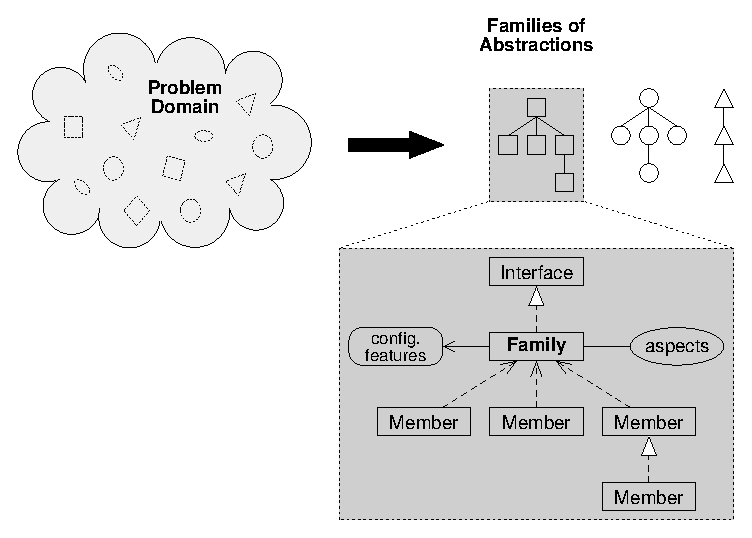
\includegraphics[width=0.70\linewidth]{aosd.eps}\par}
\caption{Overview of application-oriented domain decomposition.}
\label{fig:aosd}
\end{figure}

\subsection*{Scenario adapters}

 As explained earlier, AOSD dictates that scenario dependencies must
 be factored out as \emph{aspects}, thus keeping abstractions
 scenario-independent. However, for this strategy to work, means must
 be provided to apply factored aspects to abstractions in a
 transparent way.  The traditional approach to do this would be
 deploying an \emph{aspect weaver}, though the \emph{scenario adapter}
 construct~\cite{Froehlich:sci:2000} has the same potentialities
 without requiring an external tool.  A scenario adapter wraps an
 abstraction, intermediating its communication with scenario-dependent
 clients to perform the necessary scenario adaptations.

\subsection*{Inflated interfaces}

 Inflated interfaces summarize the features of all members of a
 family, creating a unique view of the family as a ``super
 component''. It allows application programmers to write their
 applications based on well-know, comprehensive interfaces, postponing
 the decision about which member of the family shall be used until
 enough configuration knowledge is acquired. The binding of an
 inflated interface to one of the members of a family can thus be made
 by automatic configuration tools that identify which features of the
 family were used in order to choose the simplest realization that
 implements the requested interface subset at compile-time.

%%%%%%%%%%%%%%%%%%%%%%%%%%%%%%%%%%%%%%%%%%%%%%%%%%%%%%%%%%%%%%%%%%%%%%%
\section[HARDWARE MEDIATORS]
{HARDWARE MEDIATORS}\label{mediators}

 An operating system designed according to the premises of
 Application-Oriented System Design can be summarily viewed as sets of
 software components that can be configured, adapted and integrated in
 order to give rise to highly customized and scenario-specific
 instances of run-time support systems. However, besides all the
 benefits claimed by software component engineering, such a class of
 run-time support systems is prone to the same need for portability as
 their more conventional relatives.

 Traditional portability strategies, mainly focused in hardware
 abstraction layers~(HAL) and virtual machines~(VM), are not concerned
 with the AOSD's purposes. Being a product of a system engineering
 process (instead of a domain engineering process), these strategies
 usually build a monolithic abstraction layer that encapsulates all
 the resources available in the hardware platform without properly
 regarding the application needs. Such modeling may be a problem when
 the platforms to be interfaced are based on \textsc{SoC}s. The
 diversity of architectures and devices in these platforms lead us to
 diagnose that the traditional specification techniques for sw-hw
 interfacing are still far from the ideal
 ``plug-and-play''~\cite{Neville:2003}. In addition, whenever
 \textsc{SoC}s are built on \emph{Programmable Logic Devices} such as
 FPGAs, the hardware specifications can be modified in a short period
 of time~\cite{Rutenbar:2001}, and thus compromising much more the
 portability of the system.

 In order to deal with this dynamism and to foster the portability of
 system abstractions to virtually any architecture, a system designed
 according to the concepts of AOSD relies on the hardware mediator
 construct. As discussed in \emph{Hardware Mediators: a Portability
 Artifact for Component-Based Systems}~\cite{Polpeta:euc:2004}, the
 main idea behind this portability artifact is not to build an
 universal hardware abstraction layer or virtual machine, but
 sustaining an \emph{interface contract} between the operating system
 and the hardware. Each hardware component is mediated via its own
 mediator, thus granting the portability of abstractions that use it
 without creating unnecessary dependencies. Indeed, hardware mediators
 are intended to be mostly static-metaprograms and thus ``dissolve''
 themselves in the system abstractions as soon as the interface
 contract is met. In other words, a hardware mediator delivers the
 functionality of the corresponding hardware component through a
 system-oriented interface.

 An important element of hardware mediators are \emph{configurable
 features}, \\which designate features of mediators that can be switched
 on and off according to the requirements dictated by abstractions. A
 configurable feature is not restricted to a flag indicating whether a
 preexisting hardware feature must be activated or not. Usually, it
 also incorporates a \emph{Generic Programmed}~\cite{Musser:1989}
 implementation of the algorithms and data structures that are
 necessary to implement that feature when the hardware itself does not
 provide it. An example of configurable feature is the generation of
 CRC codes in mediators that abstract communication devices.

 Likewise abstractions in AOSD (Figure~\ref{fig:aosd}), hardware
 mediators are organized in families whose members represent
 significant entities in the hardware domain. Such modeling enables
 the generation of object-code only for those mediators that are
 necessary to support the application. Non-functional aspects and
 cross-cutting properties are factored out as \emph{scenario aspects}
 that can be applied to family members as required. For instance,
 families like \texttt{UART} and \texttt{NIC}~(\emph{Network Interface
 Card}) must often operate in exclusive-access mode. This could be
 achieved by applying a share-control aspect to the families.

%%%%%%%%%%%%%%%%%%%%%%%%%%%%%%%%%%%%%%%%%%%%%%%%%%%%%%%%%%%%%%%%%%%%%%%
\section[CO-DESIGNING WITH HARDWARE MEDIATORS]
{CO-DESIGNING WITH HARDWARE MEDIATORS\label{medcodesign}}

 Although originally devised to give rise to highly adaptable
 system- hardware interface, hardware mediators can be also used for
 generating application-oriented hardware instances. More
 specifically, in the context of programmable logic, where hardware
 components, namely soft-IPs, are described using hardware description
 languages (e.g. VHDL, VERILOG) in order to implement the elements of
 the underling hardware technology. Hence, by associating hardware
 mediators with those descriptions one can infer which hardware
 components are necessary to support the application.

 A component-based system can thus rely on hardware mediators not only
 to interface its system abstractions to the hardware, but also to
 dictate which components will build-up the target hardware. As soon
 as a hardware mediator is selected to interface a hardware component,
 the associated \textsc{IP} is selected from a repository in order to
 integrate a hardware description that will be synthesized in a
 \textsc{PLD} device. Such a description in the form of a \textsc{SoC}
 would embed only the hardware components necessary to support the
 run-time system and, in turn, the application.

 For instance, consider a family of \texttt{NIC} mediators and a
 family of \texttt{NIC} hardware components whose members are
 associated to the members of the mediator's family. From a given
 application that uses a system abstraction to implement an Ethernet
 network one can infer that a member of the family \texttt{NIC} will
 be instantiated. However, the decision of which specific member will
 be instantiated, since all members are functionally equivalent, is up
 to the application's programmer. This situation characterizes what we
 named a \emph{combined IP-selection}. The hardware devices are
 inferred considering an application requirement and a specific
 decision of the application's programmer.

 Another scenario, named \emph{discreet IP-selection}, is related to
 the selection of hardware components considering only the
 application's requirements --- no explicit programmer decision must
 be taken. A good example for this scenario is related to the memory
 management scheme that will be implemented by the run-time support
 system. Once the application programmer uses system abstractions that
 rely on a \emph{paging} scheme (e.g. \emph{multitasking}), the
 \texttt{MMU} mediator is automatically inferred and, consequently, a
 memory management unit will be selected for synthesis. Conversely,
 when a \emph{flat} memory scheme is adopted no memory management unit
 is synthesized.

 A third scenario, named \emph{explicit IP-selection}, represents the
 chance of the programmer to choose the hardware components that will
 be instantiated in the system. Even if the respective mediators are
 ``hidden'' by system abstractions, the programmer explicitly selects
 the hardware components that he is intending to embed in the
 \textsc{SoC}. Indeed, this selection strategy is always taken when
 the programmer initially specifies which architecture model
 (e.g. \texttt{SPARCV8}, \texttt{OR32}) the system will follow.

 Furthermore, the approach is not restricted to the specification of
 which \textsc{IP}s will be instantiated in a \textsc{PLD} device. The
 element \emph{configurable feature} explained earlier can be also
 deployed on hardware components. They can be used to configure
 \textsc{IP}s in order to properly support the application and also to
 switch on and off some functionalities that can be implemented in
 hardware or in software. As exemplified earlier with CRC codes, a
 configurable feature can be used to enable the generation of these
 codes in a \texttt{UART} mediator for data transmitted over a serial
 communication line. Such codes, otherwise, could be generated by the
 hardware itself instead of the software. In this case, since the
 \textsc{IP} that implements the \texttt{UART} device supports
 generation of CRC codes, a hardware configurable feature would be
 activated in order to enable the synthesis of these functionalities
 in the \textsc{SoC}.

%%%%%%%%%%%%%%%%%%%%%%%%%%%%%%%%%%%%%%%%%%%%%%%%%%%%%%%%%%%%%%%%%%%%%%%
\section[CASE STUDY: SOCS IN EPOS]
{CASE STUDY: SOCS IN EPOS\label{epos}} 

 The Embedded Parallel Operating System~(\textsc{Epos}) aims at
 delivering adequate run-time support for dedicated computing
 applications. Relying on the \emph{Application-Oriented System
 Design} method, \textsc{Epos} consists of families of software
 components that can be adapted to fulfill the requirements of
 particular applications. In order to maintain the portability of its
 systems abstractions and to enable the generation of
 application-oriented \textsc{SoC}s, the \textsc{Epos} system relies
 on the hardware mediator construct.

 An application written on \textsc{Epos} can be submitted to a tool
 that scans it searching for references to the \emph{inflated
 interfaces}, thus rendering the features of each family that are
 necessary to support the application at run-time. This task is
 accomplished by a tool, the analyzer, that outputs an specification
 of requirements in the form of partial component interface
 declarations, including methods, types and constants that were used
 by the application.

 The primary specification produced by the analyzer is subsequently
 fed into a second tool, the configurator, that consults a build-up
 database to create the description of the system's
 configuration. This database holds information about each component
 in the repository, as well as dependencies and composition rules that
 are used by the configurator to build a dependency three. The output
 of the configurator consists of a set of keys that define the binding
 of inflated interfaces to abstractions and activate the scenario
 aspects eventually identified as necessary to satisfy the constraints
 dictated by the target application or by the configured execution
 scenario. On the side of the hardware components, the configurator
 produces a list of instantiated mediators and specifies which of
 these mediators promote \textsc{IP} synthesis.

\begin{figure}{
\centering
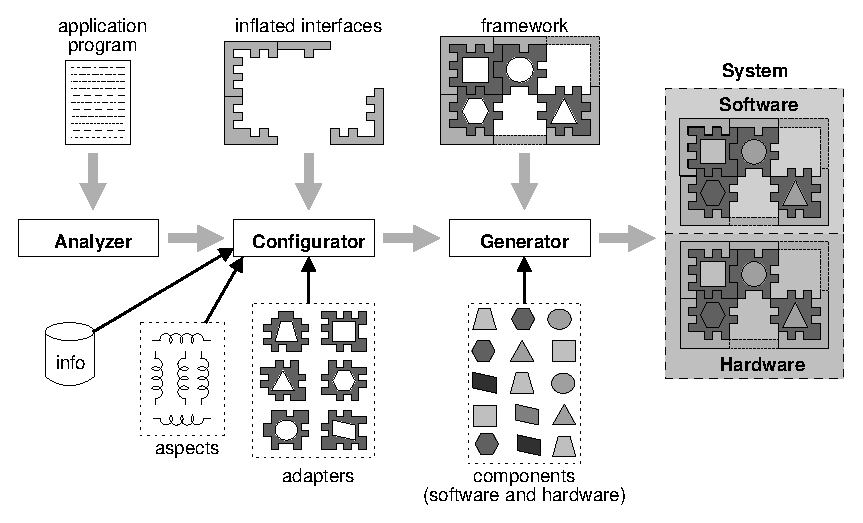
\includegraphics[width=0.76\linewidth]{epos_overview.eps}\par}
\caption{An overview of the tools involved in the automatic generation of 
run-time support and hardware instances.}
\label{fig:epos_overview}
\end{figure}

 The last step in the generation process is accomplished by the
 generator. This tool translates the keys produced by the configurator
 into parameters for a statically metaprogramed component framework
 and causes the compilation of a tailored operating system
 instance. In addition, whenever a \textsc{SoC} needs to be tailored,
 the \texttt{generator}, based on the \textsc{IP} configurable
 features, produces a synthesis configuration file. This file, as well
 as the selected \textsc{IP}s, are passed to a third-party tool, which
 in turn performs the synthesis of a \textsc{SoC}. An overview of the
 whole procedure is depicted in Figure~\ref{fig:epos_overview}.

%%%%%%%%%%%%%%%%%%%%%%%%%%%%%%%%%%%%%%%%%%%%%%%%%%%%%%%%%%%%%%%%%%%%%%%%%%

\subsection{Sample Instance: Leon SoCs in EPOS}

 In order to evaluate our approach for automating the design of
 SoC-based embedded systems we used the \emph{Leon2 Processor}. This
 ``processor'' was created in order to enable the development of
 customized SoCs based on the SPARCV8 CPU core. The ``modular'' design
 of \textsc{Leon2} enable us to specify which of its \textsc{IP}s will
 be synthesized in the \textsc{SoC}. The logic necessary to glue the
 \textsc{IP}s is implicitly defined in the source-code through a set
 of programming asserts, which are, in turn, used to properly
 configure and plug-in the \textsc{IP}s in a \textsc{Amba} bus
 framework~\cite{AMBA}. The Figure~\ref{fig:leon2}(a) shows the block
 diagram of \textsc{Leon2}. Besides the \texttt{CPU} core,
 \textsc{Leon2} includes a set of peripherals that can be plugged in
 as soon as the user selects them.

\begin{figure}{
\centering
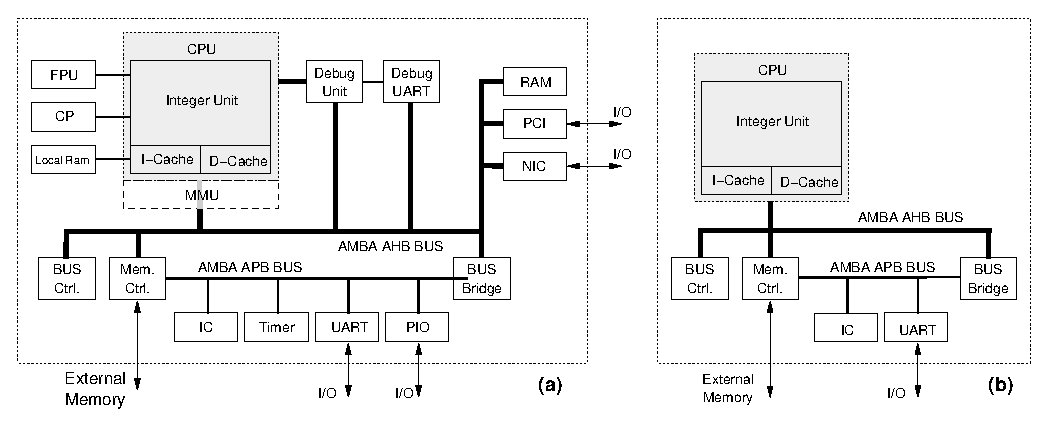
\includegraphics[width=1.0\linewidth]{leon2.eps}\par}
\caption{Block diagram of Leon2 (a) and the SoC that was experimentally 
customized (b).}
\label{fig:leon2}
\end{figure}

 The experiments were performed on a Xilinx Virtex2 FPGA development
 kit and consisted of evaluating an application for which a run-time
 support system and a \textsc{SoC} should be generated. The
 application implemented two threads, \emph{TX} and \emph{RX}, which
 were executed in a cooperative environment in order to send and
 receive data through an \texttt{UART}. Aiming at signaling the
 \emph{RX} thread to deal with new data in the \textsc{UART} buffer
 the mechanism of \emph{interrupts} was used. Consequently, the
 mediator and the \textsc{IP} of the interrupt
 controller~(\texttt{IC}) were selected to be instantiated. As regards
 the memory management scheme, it was based on a \emph{flat}
 address-space and therefore, no \textsc{MMU} components were
 instantiated in the system. The Figure~\ref{fig:leon2}(b) depicts the
 block diagram of the \textsc{SoC} that was generated after submit the
 application to the sequence of tools presented in section~\ref{epos}.

 Aiming at clarifying the expressiveness of this sample instance, it
 is important to compare the obtained results to the numbers of
 ordinary operating system that were ported to the \textsc{Leon2}
 platform. Usually these systems are generated to compromise all the
 features that the \textsc{SoC} is able to provide. The absence of a
 component-based engineering and the lack of modern software
 engineering techniques affects not only the size and performance of
 the final system, but also effectively increase NRE costs and
 time-to-market. For instance, the \textsc{Epos} instance generated to
 support the experimental application was 2.94 Kbytes and the
 associated \textsc{SoC} (Figure~\ref{fig:leon2}(b)) took 29\% of the
 Virtex2 FPGA area. Traditional ports of
 \textsc{uCLinux}~\cite{LeonuClinux:2003} and
 \textsc{eCos}~\cite{Massa:2002} to the Leon2 platform have,
 respectively, 2,740 and 432.94 Kbytes each and the both were ported
 to a SoC instance with 13,261 LUTs~(\emph{Look-up-Table}), which
 represents 60\% of the Virtex2 area.

%%%%%%%%%%%%%%%%%%%%%%%%%%%%%%%%%%%%%%%%%%%%%%%%%%%%%%%%%%%%%%%%%%%%%%%%%%

\section[CONCLUSION AND FUTURE WORK]
{CONCLUSION AND FUTURE WORK}

 In this article we conjectured about the the use of \emph{hardware
 mediators} as a new co-design artifact. The deployment of
 \textsc{AOSD} in the context where mediators were originally proposed
 leaded us to use this portability artifact for the automatic
 generation of SoC-based embedded systems. The presented results are
 quite simple and just showed the viability of generating run-time
 support systems and system-on-chip instances considering the
 application's requirements. However, as exemplified in the
 section~\ref{medcodesign}, we are not only able to identify which
 devices shall be instantiated in the \textsc{SoC} but, in fact, to
 configure each system component in order to better fits the
 application's requirements. In this sense a large gamma of new
 experiments started to be evaluated, such as processor scalability,
 memory hierarchy exploration and power management. The results
 obtained so far are encouraging and we hope present them soon.
 
%%%%%%%%%%%%%%%%%%%%%%%%%%%%%%%%%%%%%%%%%%%%%%%%%%%%%%%%%%%%%%%%%%%%%%%%%%

\begin{chapthebibliography}{1}

\bibitem{AMBA}
ARM (2003).
\newblock {\em The de facto Standard for On-Chip Bus}.
\newblock Advanced RISC Machines Limited, online document edition.
\newblock http://www.arm.com/ products/ solutions/ AMBAHomePage.html.

\bibitem{Bergamaschi:2001}
Bergamaschi, R.~A., Bhattacharya, S., Wagner, R., Fellenz, C., Muhlada, M.,
  Lee, W.~R., White, F., and Daveau, J.-M. (2001).
\newblock Automating the design of SoCs using cores.
\newblock {\em IEEE Des. Test}, 18(5):32--45.

\bibitem{Booch:1994}
Booch, G. (1994).
\newblock {\em Object-Oriented Analysis and Design with Applications}.
\newblock Addison-Wesley, 2nd edition.

\bibitem{Froehlich:2001}
Frohlich, A.~A. (2001).
\newblock {\em Application-Oriented Operating Systems}.
\newblock Number~17 in GMD Research Series. GMD - Forschungszentrum
  Informationstechnik, Sankt Augustin.

\bibitem{Froehlich:sbac:1999}
Fr\"ohlich, A.~A. and Schr\"oder-Preikschat, W. (1999).
\newblock High performance application-oriented operating systems -- the epos
  aproach.
\newblock In {\em Proceedings of the 11th Symposium on Computer Architecture
  and High Performance Computing}, pages 3--9, Natal, Brazil.

\bibitem{Froehlich:sci:2000}
Fr\"ohlich, A.~A. and Schr\"oder-Preikschat, W. (2000).
\newblock Scenario adapters: Efficiently adapting components.
\newblock In {\em Proceedings of the 4th World Multiconference on Systemics,
  Cybernetics and Informatics}, Orlando, U.S.A.

\bibitem{Habermann:1976}
Habermann, A.~N., Flon, L., and Cooprider, L. (1976).
\newblock Modularization and hierarchy in a family of operating systems.
\newblock {\em Commun. ACM}, 19(5):266--272.

\bibitem{Kiczales:1997}
Kiczales, G., Lamping, J., Mendhekar, A., Maeda, C., Lopes, C.~V., Loingtier,
  J.-M., and Irwin, J. (1997).
\newblock Aspect-oriented programming.
\newblock In {\em Proceedings of the European Conference on Object-oriented
  Programming'97}, volume 1241 of {\em Lecture Notes in Computer Science},
  pages 220--242, Jyv skyl, Finland. Springer.

\bibitem{LeonuClinux:2003}
Wurm, M. (2003).
\newblock uClinux for sparc-mmuless with ethernet mac.
\newblock Technical report, Graz University of Technology.

\bibitem{Massa:2002}
Massa, A. (2002).
\newblock {\em Embedded SW. Development with eCos}.
\newblock Prentice Hall, 1st edition.

\bibitem{Mattsson:2004}
Mattsson, D. and Christensson, M. (2004).
\newblock Evaluation of synthesizable cpu cores.
\newblock Technical report, Chalmers University Of Technology.

\bibitem{Mikhajlov:1998}
Mikhajlov, L. and Sekerinski, E. (1998).
\newblock A study of the fragile base class problem.
\newblock In {\em Proceedings of the 12th European Conference on
  Object-Oriented Programming}, pages 355--382. Springer-Verlag.

\bibitem{Musser:1989}
Musser, D.~R. and Stepanov, A.~A. (1989).
\newblock Generic programming.
\newblock In {\em Proceedings of the First International Joint` Conference of
  ISSAC and AAECC}, number 358 in Lecture Notes in Computer Science, pages
  13--25, Rome, Italy. Springer.

\bibitem{Neville:2003}
Neville-Neil, G. and Whitney, T. (2003).
\newblock Soc: Software, hardware, nightmare, bliss.
\newblock {\em ACM Queue}, 1(2):24.

\bibitem{Parnas:1976}
Parnas, D.~L. (1976).
\newblock On the design and development of program families.
\newblock {\em IEEE Transactions on Software Engineering}, SE-2(1):1--9.

\bibitem{Polpeta:euc:2004}
Polpeta, F.~V. and Fr\"ohlich, A.~A. (2004).
\newblock Hardware mediators: a portability artifact for component-based
  systems.
\newblock In {\em Proceeding of the International Conference on Embedded and
  Ubiquitous Computing}, volume Lecture Notes in Computer Science, pages
  271--280, Aizu,Japan. Springer.

\bibitem{Rutenbar:2001}
Rutenbar, R.~A., Baron, M., Daniel, T., Jayaraman, R., Or-Bach, Z., Rose, J.,
  and Sechen, C. (2001).
\newblock (When) Will FPGAs kill ASICs?
\newblock In {\em Proceedings of the 38th conference on Design automation},
  pages 321--322. ACM Press.

\end{chapthebibliography}

\end{document}

